\chapter{Entwurf der Benutzerschnittstelle}\label{chapter_4}
Die Anforderungen der Anwendung für die Unterstützung des neuen Workflows wurden im vorigen Kapitel abgeleitet. Diese Kriterien werden im nächsten Schritt in einem Entwurf der Benutzerschnittstelle umgesetzt. Bevor die Schnittstelle entworfen werden kann, muss die geeignete Anwendungsform und eine darauf basierende Technologie ausgewählt werden. Anschließend folgt eine kurze Analyse der Zielplattform und deren Konzepte, damit diese beim Entwurf berücksichtigt werden können, bevor die einzelnen Ansichten entworfen werden.

\section{Auswahl der Anwendungsplattform}
Aufgrund der vielen Möglichkeiten bei der Entwicklung von mobilen Anwendungen muss die Art und Technologie der Anwendung richtig gewählt werden. Hierbei soll zuerst die passende Anwendungsform (Nativ, Web oder Hybrid siehe \ref{mobileAppsGrundlagen}) gewählt werden. Durch diese Vorauswahl, wird die Anzahl der möglichen Technologien begrenzt, was im folgenden Schritt die Auswahl vereinfacht.


\subsection{Anwendungsform}
Damit die richtige Anwendungsform der App ausgewählt werden kann, müssen die drei Möglichkeiten Nativ, Web und Hybrid auf ihre Eignung bei der Umsetzung der Anforderungen untersucht werden. Wichtig bei der Entscheidung ist die Festlegung der konkreten Kriterien. 
Die Umsetzung der rein fachlichen Funktionen Produktauswahl und Konfiguration kann mit jeder Anwendungsform durchgeführt werden. Hier sind die Unterschiede für eine Auswahl nicht ausreichend. \par
Bei den  Funktionalen Anforderungen sind die zwei Kriterien, die aufgrund der mobilen Zielumgebung wichtig sind für die Auswahl bedeutend. Diese sind das Speichern und Laden (F5), sowie die Filterung der Anwendungsdaten (F6). Für die Umsetzung dieser Funktionen ist eine Verwendung des Dateisystems auf der mobilen Zielumgebung notwendig. Hier muss eine Form der Speicherung, ob Datenbank oder einfaches Speichern in einer Datei möglich sein. Diese Voraussetzung ist für die Entscheidung der Anwendungsform essentiell. \par

Das zweite Kriterium leitet sich von den Nicht-Funktionalen Anforderungen einer schnellen Bedienung (N2) ab. Damit die Anwendung schnell bedient werden kann, müssen die vorhandenen Hardwareressourcen optimal verwendet werden können. Dies ist notwendig, um bspw. das Laden von Bildern zu beschleunigen. Ebenfalls müssen Seitenübergänge ohne große Wartezeiten möglich sein, um die Anforderung erfüllen zu können. Die Anwendungsform muss für die Umsetzung Schnittstellen bereitstellen, die auf die vorhandene Hardware optimiert sind.

Für eine Optimierung der Anwendung auf die Zielumgebung (N3) ist ein ästhetisches und minimalistisches Design die entscheidende Heuristik für die Auswahl der Anwendungsform. Für die Implementierung muss eine gute optische Integration in das System vorhanden sein. Dies ist für eine übersichtliche Aufbereitung des Produktkataloges eine Voraussetzung. Der App-Typ muss Oberflächenelemente zur Verfügung stellen, die zu der Gesamtumgebung passen. Durch eine gute Integration in die Zielumgebung wird dadurch die Anwendung ästhetischer. Die gesamte Wahrnehmung der App wird hierdurch verbessert. Das dritte Zielkriterium für die Auswahl ist somit die Verwendung von betriebssystemspezifischen Oberflächenelementen.    

Im Folgenden werden die drei festgestellten Kriterien lokale Speicherung der Daten, Hardwarenahe Schnittstellen und Verwendung von betriebssystemspezifischen Oberflächenelementen  für jede Anwendungsform bewertet, sodass am Ende eine Gegenüberstellung stattfinden kann.

\paragraph{Native Anwendung: }Bei Nativen Anwendungen ist der komplette Funktionsumfang der mobilen Zielplattform verfügbar. Dies ermöglicht ein breites Anwendungsfeld für native Anwendungen.
\begin{itemize}
\item \textbf{Lokale Speicherung der Daten:} Die native Anwendungsform stellt Schnittstellen für den Zugriff auf eine lokale Datenbank oder ein lokales Dateisystem bereit. Diese können ohne Anpassungen verwendet werden. 

\item \textbf{Hardwarenahe Schnittstellen:} Dadurch, dass die einzelnen Schnittstellen direkt vom Hersteller der jeweiligen Plattform kommen, sind Operationen für das System optimiert. Mit einer nativen Anwendung wird damit die beste Performanz erreicht. 

\item \textbf{Betriebssystemspezfische Oberflächenelemente:} Native Anwendungen verwenden für die Benutzerschnittstelle die spezifische Oberflächenelemente. Die Steuerung mit Touch ist ebenfalls auf diese Anwendungsform optimiert. Dies ergibt eine vollständige Verwendungsmöglichkeit des bereitgestellten Frameworks.
\end{itemize}

Auf die einzelnen Kriterien bezogen erfüllt die native Anwendung alle Anforderungen. Der volle Funktionsumfang des Systems ist gegeben, wodurch die App ideal für die gewählte Zielplattform geeignet ist.

\paragraph{Web Anwendung: } Web Anwendungen werden im Browser ausgeführt. 
 Dies führt dazu, dass nur Funktionen verwendet werden können, die der jeweilige Browser auf der Zielplattform zur Verfügung stellt. 
 \begin{itemize}
 \item \textbf{Lokale Speicherung der Daten:} Ein Speichern und Laden der Daten vom Betriebssystem ist bei einer Web Anwendung nicht ohne weiteres möglich. Der Browser verbietet durch das Sandbox-Modell einen direkten Zugriff auf das System.  Ein Ansatz zur Lösung des Problems ist die Installation des Servers direkt auf dem Zielsystem, so dass dieser lokal zur Verfügung steht. Eine Erfüllung der Anforderungen ist damit möglich, jedoch mit erheblichem Mehraufwand. 
 
 \item \textbf{Hardwarenahe Schnittstellen:} Die Kommunikation mit dem Betriebssystem erfolgt durch den Browser. Diese zusätzliche Zwischenschicht sorgt dafür, dass die Hardware nicht direkt verwendet wird, wie es bei einer nativen Anwendung der Fall ist. Der zusätzliche Overhead sorgt dafür, dass die Performance bei einer Web Anwendung nicht ideal im Vergleich zur nativen Lösung ist.
 
 \item \textbf{Betriebssystemspezfische Oberflächenelemente:} Die grundlegenden Oberflächenelemente sind HTML Elemente. Diese können mit Javascript und CSS einen passenden Stil für das jeweilige Betriebssystem erhalten. Die Verwendung von speziellen Touch Gesten ist mit Web Anwendungen aufgrund der Interoperabilität mit mehreren Betriebssystemen schwieriger. Hier sind ebenfalls nur begrenzte Interaktionen möglich.
 
 \end{itemize}
 Der Hauptvorteil der Web Anwendung die Verwendung, ohne komplette neue Implementierung auf mehreren Systemen ist aufgrund der Kriterien nicht relevant. Die wichtigen Eigenschaften der Anwendung Performanz und lokale Speicherung können mit dieser Anwendungsform gelöst werden, jedoch deutlich schlechter als bei der nativen Variante.


\paragraph{Hybride Anwendung: }Durch die Verwendung der lokalen Schnittstellen im nativen Anwendungscontainer (siehe \ref{hybridApplication}) können die vorhanden Ressourcen wie bei einer Nativen Anwendung verwendet werden. Dies führt zu einigen Verbesserungen gegenüber einer reinen Web Anwendung.

\begin{itemize}
 \item \textbf{Lokale Speicherung der Daten:} Für die Umsetzung dieser Anforderung muss eine geeignete Schnittstelle im Anwendungscontainer zur Verfügung gestellt werden. Hierdurch wird eine problemlose Verwendung des Dateisystems möglich. Das Kriterium kann ohne Einschränkungen erfüllt werden. 
 
 \item \textbf{Hardwarenahe Schnittstellen:} Durch den Anwendungscontainer wird, wie bei einer Webanwendung der Browser, eine Zwischenschicht nötig. Damit wird ein zusätzlicher Kommunikationsaufwand benötigt. Dieser zusätzliche Aufwand verringert die Performanz der Anwendung.
 
 \item \textbf{Betriebssystemspezfische Oberflächenelemente:} Die Oberflächenelemente des Betriebssystems lassen sich im Container bereitstellen. Somit können die nativen Elemente in der Hybriden Anwendung verwendet werden. Die Verwendung der Touch Bedienung wird durch dieses Konzept ermöglicht.
 \end{itemize}
 Die Probleme, die bei der Verwendung einer Web Anwendung auftreten können durch den hybriden Ansatz gelöst werden. Ein Problem was weiterhin besteht, ist die Performanz. Diese wird mit der hybriden Anwendungsform besser, kommt jedoch nicht an die Leistung einer nativen Anwendung heran.

\paragraph{Abwägung: }

Nachdem alle Anwendungsformen auf die Erfüllung der aufgestellten Kriterien untersucht sind, kann eine Gegenüberstellung der einzelnen Komponenten erfolgen. Die Tabelle \ref{decision} zeigt eine Bewertung der Kriterien. Hierbei wurden die einzelnen Punkte anhand einer Skala von 0 (kann nicht erfüllt werden) bis 5 (ohne Einschränkungen möglich) bewertet.  Die Implementierung als Web Anwendung scheidet klar aus. Die Anforderungen können zwar umgesetzt werden, jedoch ist ein erheblicher Mehraufwand für die Erreichung nötig. Ebenfalls hat die Anwendung im Vorhinein bereits Einschränkungen bzgl. der Performanz, sowie der Bereitstellung von Oberflächenelementen. Die Vorteile einer Implementierung für mehrere Zielsysteme ist bei der Umsetzung kein Kriterium. \par
\begin{figure}
\begin{tabular}{| p{5.4cm} | p{2.5cm} | p{2.5cm} | p{2.5cm} |}
\toprule[2pt] \rowcolor{dunkelgrau}
\hline
  Kriterium & Web \newline Anwendung & Hybride \newline Anwendung & Native \newline Anwendung \\
  \hline
  Lokale Datenspeicherung & 1 & 4 & 5
   \\
  \hline
  Hardwarenahe Schnittstellen &1  &2  & 5  \\
  \hline
    Betriebssystemspezifische Oberflächenelemente & 1 & 4 & 5 \\
  \hline
    Summe & 3 & 10 & 15 \\
  \hline
\bottomrule[2pt]
\end{tabular}
\caption{Gegenüberstellung und Bewertung der Zielkriterien für die Anwendungsform}
\label{decision}
\end{figure}
\par 
Schwieriger ist die Entscheidung zwischen hybrid und nativ. Die beiden Kriterien lokale Speicherung der Daten und betriebssystemspezifsche Oberflächenelemente sind mit beiden Ansätzen ohne größere Einschränkungen möglich. Beim hybriden Ansatz ist ein geringer Mehraufwand bei der Implementierung nötig. Dies ist jedoch nicht relevant für die Entscheidung. Der wichtigste Grund für die Entscheidung für eine nativen Anwendung ist die Performanz bei der Bedienung. Nur durch die Verwendung von nativen Anwendungen können aufwändige Animationen oder das Rendern von vielen Bildern flüssig ablaufen. Eine hybride Lösung besitzt hier Einschränkungen, da die Hardware mit einer Zwischenschicht verwendet wird.

\subsection{Anwendungstechnologie}
Mit der Entscheidung für eine mobile Anwendungsform kommen drei mögliche Technologien für die Implementierung in Frage. Die Plattformen Android \footnote{http://www.android.com/}, iOS \footnote{http://www.apple.com/de/iphone/ios/} und Windows 8 \footnote{http://windows.microsoft.com/de-de/windows-8/} sind aufgrund ihrer Marktanteile (Android: 43,4\% iOS: 48,2\% Windows: 7,4\% Quelle: \cite{bib:marktanteilBS} ) die wichtigsten Technologien im Tablet Bereich. Die drei Plattformen haben unterschiedliche Ziele. Das iOS Betriebssystem hat den Vorteil einer hohen Verbreitung bei Business Anwendungen (siehe \cite[S.5]{bib:mobileMarketing2}). Android hat die meisten Nutzer bei Privatanwendungen (siehe \cite{bib:marktanteilMBS}). Bei Windows 8 ist der Vorteil eines neuen Konzeptes, was speziell für Tablet-PCs optimiert ist. Für die Umsetzung des Workflows kann jede dieser Technologien verwendet werden, da die Zielkriterien sich bei den unterschiedlichen Plattformen nicht unterscheiden (siehe Tabelle \ref{decisionTechnologie}). Ist die Implementierung mit einem Framework umgesetzt, stellt das Implementieren auf einer anderen Zielplattform keine Herausforderung dar. \par 
\begin{figure}
\begin{tabular}[H]{| p{5.4cm} | p{2.5cm} | p{2.5cm} | p{2.5cm} |}
\toprule[2pt] \rowcolor{dunkelgrau}
\hline
  Kriterium & Android & iOS & Windows 8 \\
  \hline
  Lokale Datenspeicherung & 5 & 5 & 5
   \\
  \hline
  Hardwarenahe Schnittstellen &4  &5  & 5  \\
  \hline
    Betriebssystemspezifische Oberflächenelemente & 5 & 5 & 5 \\
  \hline
    Summe & 14 & 15 & 15 \\
  \hline
\bottomrule[2pt]
\end{tabular}
\caption{Gegenüberstellung und Bewertung der Zielkriterien für Plattform}
\label{decisionTechnologie}
\end{figure}

Bei der vorliegenden Arbeit wird auf Windows 8 gesetzt. Im Gegensatz zu iOS und Android wird dieses Betriebssystem nicht auf Smartphones ausgeführt. Dies führt zu einer besseren Optimierung für größere Bildschirme. Die Technologie ist sehr neu auf dem Markt (26. Oktober 2012), dadurch gibt es noch nicht viele Apps. Dies bietet die Möglichkeit den Anwender mit neuen Möglichkeiten in der Anwendung zu überraschen, da einige Konzepte noch nicht bekannt sind. Die Möglichkeit zu experimentieren und neue Ideen umzusetzen ist aufgrund der neuen Plattform vorhanden.  Die Verwendung von Windows 8 vereinfacht ebenfalls die Integration in ein Unternehmensumfeld, da hier die Microsoft Produkte weit verbreitet sind. Dies führt zu einer schnelleren Akzeptanz im Unternehmen. Somit wird im Folgenden die Anwendung für das Windows 8 Betriebssystem implementiert.
        

\section{Untersuchung der Plattform Windows 8}
Damit die Anforderung eines ästhetischen und minimalistischen Designs (N3) erfüllt ist, muss vor der Gestaltung der einzelnen Ansichten die Zielplattform untersucht werden. Die Designgrundlagen müssen verstanden werden, um ein passendes Aussehen realisieren zu können. 
Die Folgende Untersuchung wird in drei Teile aufgeteilt. Im ersten Abschnitt werden allgemeine Design Prinzipien behandelt, darauf aufbauend die Bedienkonzepte und touchoptimierten Bedienelemente der Plattform.

\subsection{Design Richtlinien}
Damit einheitliche Apps entwickelt werden, hat Microsoft Richtlinien (Entnommen aus: \cite{bib:win80}, \cite{bib:win81}, \cite{bib:win82}, \cite{bib:win83}) aufgestellt.
Das wichtigste Design Element bei einer Windows 8 Anwendung sind sogenannte Kacheln. Diese Kacheln sind meist quadratisch und in jeder App vorhanden . Jede Funktion wird über eine Kachel erreicht. Sie soll mehr Informationen darstellen, als ein einfaches Logo oder Icon auf einem Button. Durch einen dynamischen Inhalt und unterschiedliche Größen wird dadurch dem Benutzer ein neues Benutzererlebnis gegeben. Die Organisation der Kacheln erfolgt in einem sogenannten Grid (engl. für Gitter). Dieses besteht aus mehreren Quadraten. Das kleinste Quadrat hat eine Größe von einem Pixel. Das Grid besitzt verschiedene Bereiche für die Überschrift und den Inhalt. Dieser ist vorgegeben und sollte eingehalten werden. \par 

Die Anwendung muss sich auf die Anzeige des Wesentlichen konzentrieren. Microsoft nennt  das Prinzip "'Content over Chrome"'.  Für die Umsetzung dieser Richtlinie soll die Anwendung nur die wichtigsten Funktionen in der Ansicht darstellen. Es sollen überladene Ansichten vermieden werden und stattdessen bewusst größere Elemente mit mehr Platz verwendet werden. 
 
Ein weiteres wichtiges Design Element ist die Typographie. Hier geht es um die bewusste Gestaltung von Schriften. Die Kalligrafie wird als Vorbild verwendet.  Die Idee ist keine rein statische Verwendung der Texte. Der Nutzer soll die Möglichkeit haben diese auszuwählen, damit eine Interaktion ermöglicht wird. 

Diese Richtlinien werden beim Entwurf der einzelnen Ansichten berücksichtigt. 


\subsection{Bedienkonzepte}\label{usingConcepts}
Bei den Konzepten für die Bedienung steht bei Windows 8 eine besondere Optimierung für Tablet-PCs im Vordergrund. Es werden deshalb sehr viele Gesten verwendet. Eine wichtige Geste ist das sogenannte "'wischen"'. Diese Aktion ist von jeder Seite des Bildschirms erlaubt. Beim Wischen von oben oder unten wird die sogenannte AppBar eingeblendet. Diese Bar wird an der oberen Seite für die Navigation durch die Anwendung verwendet. Dies ermöglicht einen schnellen Wechsel zwischen den Ansichten. Die untere AppBar wird für Aktionen verwendet, die nicht Vordergrund stehen. Ein Beispiel wäre die Filterung der Eingabedaten nach bestimmten Kriterien. Ein Wischen von der rechten Seit lässt die sogenannte CharmBar erscheinen. Der Inhalt dieser Bar ist die Verwendung von sogenannten Contracts (engl. Verträge). Diese Funktionen werden für alle Anwendungen durch das Betriebssystem bereitgestellt. An dieser Stelle können Einstellungen oder Suchen durchgeführt werden. \par 

Das zweite wichtige Bedienkonzept ist das horizontale Scrollen. Aufgrund der größeren Bedienelemente sind nicht immer alle Elemente sichtbar. Die Lösung ist ein horizontales Ausbreiten des Inhalts. Damit die Inhalte verwendet werden können, wird ein horizontales Scrollen mit einer Wisch-Geste durchgeführt. Hier muss darauf geachtet werden, dass ein Ausschnitt des nächsten Elementes sichtbar ist, damit dem Benutzer eine Erweiterung der Ansicht signalisiert wird. \par 

Beim Aufbau der Anwendung kann entweder eine hierarchische oder  flache Struktur verwendet werden. Für den in Abschnitt \ref{workflowNew} erstellen Workflow ist eine hierarchische Architektur passender. Der Ursprung geht hier immer von der Startseite, der sogenannten Hub-Page aus. Diese Seite ist der zentrale Startpunkt von der alle weiteren Aktionen ausgehen. Die zweite Ebene sind sogenannte Section Pages. Diese stellen den Inhalt einer  Kategorie dar. Die unterste Ebene sind die Detail Pages. Diese enthalten die jeweiligen Details eines Elementes in einer Kategorie. Bei einer Zeitungs App wäre beispielsweise auf der Startseite die einzelnen Kategorien wie Politik, Wirtschaft oder Sport zu sehen. In der Kategorie Ansicht die jeweiligen Überschriften der Artikel. Die Detail Seite würde den Artikel zeigen. Dieser baumartige Aufbau wird durch das Verwenden eines Zurück Buttons unterstützt, der in jeder Ansicht, außer der Startseite vorhanden ist. Durch diesen Button wird dem Benutzer eine weitere Navigationsmöglichkeit gegeben.

Beim Design der Ansichten ist ein durchdachtes Bedienkonzept aufgrund der beiden Anforderungen N1 und N2 wichtig. Die Möglichkeiten, die zur Verfügung gestellt werden, sollten beim ersten Entwurf der App enthalten sein.

\subsection{Touchoptimierte Bedienelemente}
Für die Unterstützung der Bedienung durch Gesten enthält das Framework besondere Oberflächenelemente. Diese sind für die Verwendung mittels Touch optimiert. Die in der Arbeit verwendeten Elemente werden im folgenden vorgestellt.
Die Design Richtlinien von Microsoft erzeugen Probleme bei der Darstellung von vielen Daten. Eine Umsetzung der Richtlinie "'Content over Chrome"', sowie die Darstellung auf einem Gerät mit kleinerem Bildschirm verursachen einen großen Aufwand beim Scrollen. Hier kann eine lange Zeit für das Auswählen eines bestimmten Datums benötigt werden. \par

Für die Lösung dieses Problems bietet Windows 8 den sogenannten Semantischen Zoom an. Diese Funktion wird mit einer Kneif-Geste auf dem aktuellen Datensatz durchgeführt. Hierdurch wird die Ansicht nicht optisch verkleinert. Es erfolgt ein Wechsel von der Detailansicht zu einer Kategorieansicht. Die Datensätze werden somit semantisch verkleinert, wodurch ein schnelles Navigieren zum gewünschten Datum möglich ist. Der Semantische Zoom darf nicht geschachtelt verwendet werden und ist damit auf eine Ebene beschränkt. Voraussetzung für die Verwendung des Zooms ist die Einteilung der Daten in Kategorien. Ohne diese Kategorien kann keine übergeordnete Ansicht erstellt werden.

Das zweite neue Bedienelement, welches für eine Touch-Optimierung dient, ist die sogenannte Flip-Ansicht. Mit ihr kann durch ein Wischen von der linken oder rechten Seite die Ansicht gewechselt werden. Dieses Element kann den Benutzer bei einem schnellen navigieren helfen. Es sollten jedoch nicht zu viele Elemente für den Wechsel vorhanden sein.

\section{Entwurf der Ansichten}
Die vorgestellten Konzepte der Anwendungsplattform, sowie die einzelnen Bedienelemente werden für den Entwurf der Ansichten verwendet. Der Workflow der App, wie in Abschnitt \ref{appWorkflow} beschrieben, wird hier als Grundlage verwendet. Damit alle Prozessschritte durchgeführt werden können, muss für jeden Zustand eine Ansicht vorhanden sein. Für die Umsetzung der Anforderungen aus Kapitel \ref{functionalRequirements} werden evtl. zusätzliche Benutzerschnittstellen benötigt.


\subsection{Hauptfunktion der Anwendung}
Um den Benutzer bei der Verwendung der App zu unterstützen, müssen zu Beginn die Hauptfunktionen der Anwendung erkannt werden. Diese Funktionen sollen gut platziert werden, um eine schnelle Bedienung zu ermöglichen. Die Platzierung erfolgt in der Hauptansicht, von der alle weiteren Aktion ausgehen.

Bei der vorliegenden Arbeit sind die Hauptfunktionen der Produktkatalog und die Konfiguration. Im Anwendungsbeispiel ist die Auswahl der Flugzuge eine Voraussetzung, damit konfiguriert werden kann. Aus diesem Grund gehört die Flugzeugauswahl ebenfalls zu den Hauptfunktionen. Wie im neuen Workflow modelliert, sind diese drei Funktionen von der Zusammenfassungsseite aus zugänglich. Somit ist diese Seite die Hauptfunktionsseite\par 
\begin{figure}
\centering
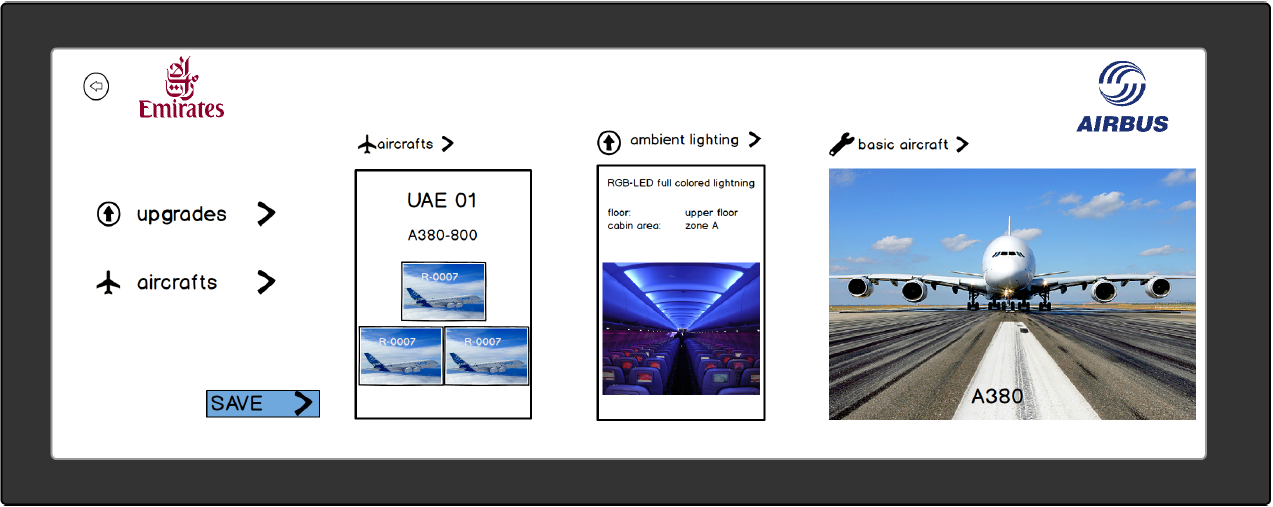
\includegraphics[width=\hsize]{images/summary_entwurf}
\caption{Entwurf der Zusammenfassung Seite}
\label{summarySketch}
\end{figure}

Der erste Entwurf der Zusammenfassung ist in Abbildung \ref{summarySketch} zu sehen. Die Hauptfunktionen Upgradeauswahl und Flugzeugauswahl sind als Buttons mit Text und Icon auf der linken Seite zu sehen. Bei der Selektion eines Buttons wird die jeweilige Ansicht der Auswahl geöffnet. Die weiteren Elemente der Zusammenfassung bestehen aus der aktuellen Auswahl. Die Darstellung erfolgt immer mit einem Bild und dem passenden Text in der Kachel Optik. Auf der ganz rechten Seite wird zuerst das ausgewählte Flugzeugprogramm angezeigt. Daneben werden die bisher ausgewählten Upgrades und Flugzeuge dargestellt. Die Reihenfolge der Darstellung hängt von der Auswahl ab. Diese werden in der gleichen Abfolge, wie zuvor ausgewählt wurde angezeigt. Damit wird das zuletzt Gewählte immer auf der linken Seite angezeigt. Bei der Zusammenfassungsseite werden die Microsoft Richtlinien für das horizontale Scrollen umgesetzt. Die einzelnen Elemente sind im Grid angeordnet.


\subsection{Produktkatalog}
Für das Verwenden der ersten Hauptfunktion, der Produktauswahl wird der entsprechende Button in der Zusammenfassung verwendet. Beim Entwurf dieser Ansicht ist die Herausforderung die übersichtliche Darstellung des Produktes. Da beim Anwendungsbeispiel ein großes und komplexes Produkt vorhanden ist, sind entsprechend viele Upgrademöglichkeiten vorhanden. Die Idee bei der Konzeption ist das Einteilen der einzelnen Upgrades in verschiedene Bereiche im Flugzeug. Beim derzeitigen Katalog sind die Upgrades bereits in Kategorien sortiert. Diese werden im Entwurf für die Einteilung auf die einzelnen Bereiche verwendet. \par

\begin{figure}[H]
\centering
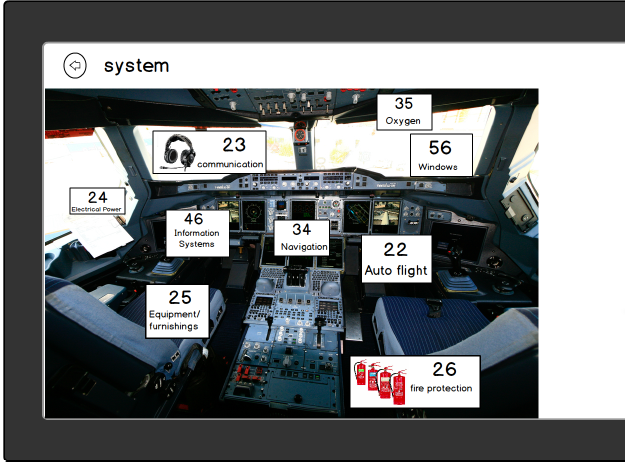
\includegraphics[width=360px]{images/catalogue_entwurf}
\caption{Entwurf der Produktkategorie Auswahl}
\label{catalogueSketch}
\end{figure}
Abbildung \ref{catalogueSketch} zeigt die Zuteilung der Kategorien auf die einzelnen Bereiche im Flugzeug. Wichtig hierbei ist das Verwenden von ansprechenden Bildern und großen Auswahlboxen. Der Kunde muss die benötigten Upgrades den einzelnen Bereichen zuordnen können und kann mit der Anwendung schnell zu seinem benötigten Produkt navigieren. Mit der Darstellung wird das Ziel erreicht, den Kunden für die Komplexität des Produktes zu sensibilisieren und ihm gleichzeitig eine bessere Suchmöglichkeit als über Produkt- oder Kategorienummern zu ermöglichen. \par 

Nach der Auswahl einer Kategorie wird nach dem in Abschnitt \ref{usingConcepts} vorgestellten Prinzip der hierarchischen Navigation eine Detail Seite angezeigt. Diese enthält die Details über die Upgrademöglichkeiten. Die Struktur beim Katalog des Anwendungsbeispiels enthält eine weitere Unterkategorie, die im Entwurf (siehe Abbildung \ref{detailSketch}) auf der linken Seite als Liste dargestellt ist. Nach der Auswahl eines dieser Elemente wird auf der rechten Seite die möglichen Upgrades der gewählten Unterkategorie angezeigt. Zusätzlich werden Informationen über die vorhandenen Möglichkeiten und optional Bilder für die Erklärung dargestellt.  Für jedes vorhandene Upgrade in einer Unterkategorie werden einzelne Kacheln verwendet. Diese können per Klick selektiert werden. Die Informationen über das jeweilige Upgrade sind in der Kachel enthalten, ebenfalls ein Produktbild und ggf. der Name des Herstellers. Diese Elemente sind immer auf dem ersten Bildschirm ohne Scrollen sichtbar. Der Benutzer sollte nur bei Bedarf von mehr Informationen scrollen müssen. Hierdurch wird eine schnelle Auswahl der gewünschten Upgrades ermöglicht. 
\begin{figure}[H]
\centering
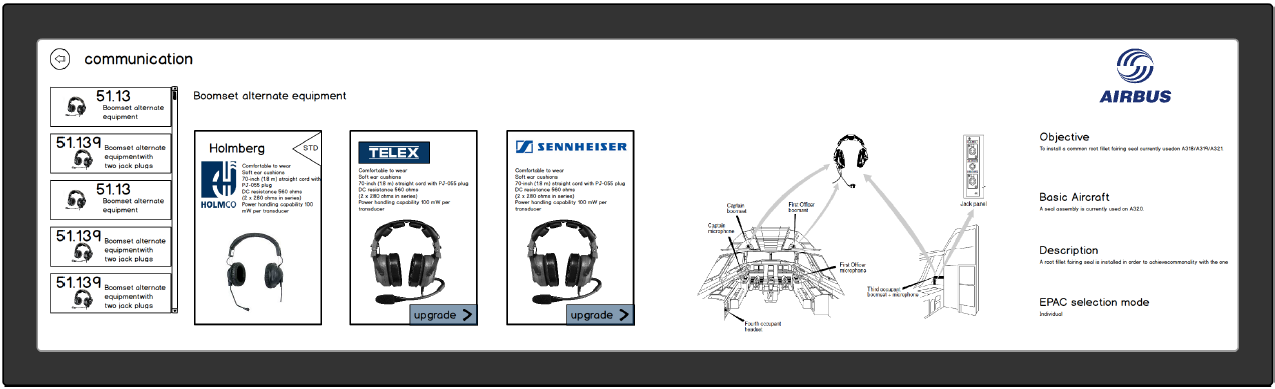
\includegraphics[width=\hsize]{images/detail_entwurf}
\caption{Entwurf der Produktdetail Ansicht}
\label{detailSketch}
\end{figure}

\subsection{Flugzeugauswahl}
Die Auswahl der Flugzeuge ist aufgrund der Voraussetzung für die Konfiguration eine Hauptaufgabe. Für eine schnelle Selektion müssen die Daten zuvor gefiltert werden. Dadurch, dass die Anwendung beim Kunden direkt verwendet wird, sind auch nur dessen Daten relevant. Der Kunde verwendet für die Auswahl die sogenannte Flugzeugversion. Bei der Bestellung von neuen Flugzeugen werden diese in eine neue Version eingeordnet. Jede Flugzeuggesellschaft erhält ein Kürzel, worauf eine Nummer für die Version folgt. Bei der Auswahl der Flugzeuge wird diese Kategorisierung beibehalten. Die vorhandenen Datenelemente werden anhand der Flugzeugversion sortiert. \par

\begin{figure}
\centering
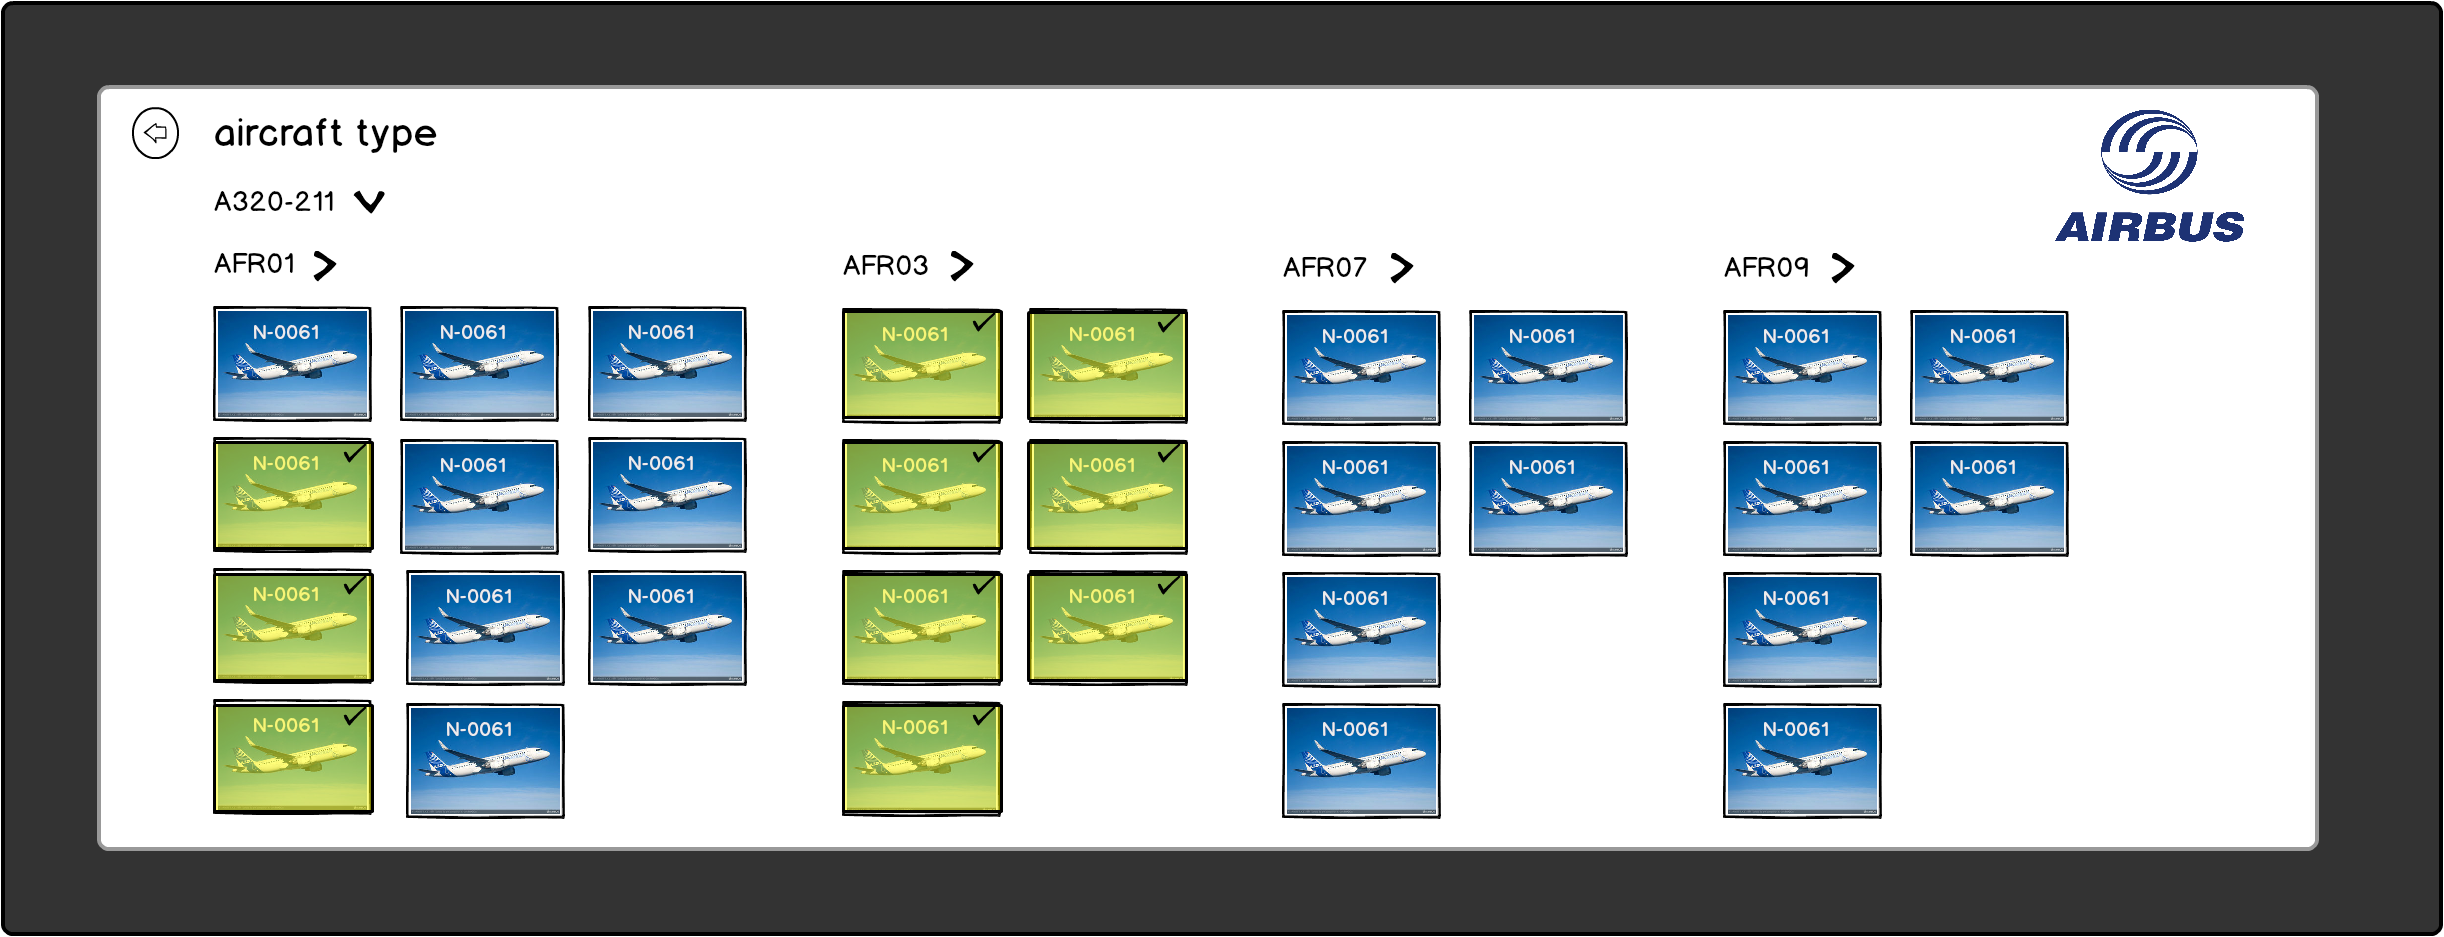
\includegraphics[width=\hsize]{images/version_entwurf}
\caption{Entwurf der Flugzeugauswahl}
\label{aircraftSketch}
\end{figure}
Die Darstellung der einzelnen Flugzeuge erfolgt, wie in Abbildung \ref{aircraftSketch} zu sehen, im Grid. Die einzelnen Flugzeuge werden in einer Kachel angezeigt, wobei jede auswählbar ist. Die Sortierung der Daten erfolgt mit den Versionen als Überschrift der jeweiligen Gruppe. Damit die Daten schneller gefunden werden können, wird ein zusätzlicher Filter verwendet. Dieser soll die Flugzeuge nach dem jeweiligen Typ filtern und so für eine besser Übersicht sorgen. Der Filter wird über den Daten platziert und soll vom Scrollen ausgeschlossen werden. \par 

Damit ein Experte beim Bedienen der Anwendung die Daten schneller auswählen kann, wie in der Funktionalen-Anforderung N2 spezifiziert, wird der Semantische Zoom für diesen Datensatz verwendet. Die herausgezoomte Ansicht enthält die Versionen als Kategorie in einem Grid dargestellt. 

\subsection{Konfigurationsergebnisse}
Die Ergebnisse der Konfiguration werden im modellierten Workflow nach erfolgter Auswahl von Ugrades und Flugzeugen angezeigt. Das Ergebnis besteht aus den gebildeten Konfigurationsgruppen. Beim Entwurf sollen die Gruppen in der Zusammenfassungsseite zu sehen sein, sobald mindestens ein Flugzeug und ein Upgrade ausgewählt wurde. Die Kommunikation mit dem Konfigurationsserver läuft hier automatisch im Hintergrund, so dass jederzeit die Ergebnisse live angezeigt werden. \par
\begin{figure}
\centering
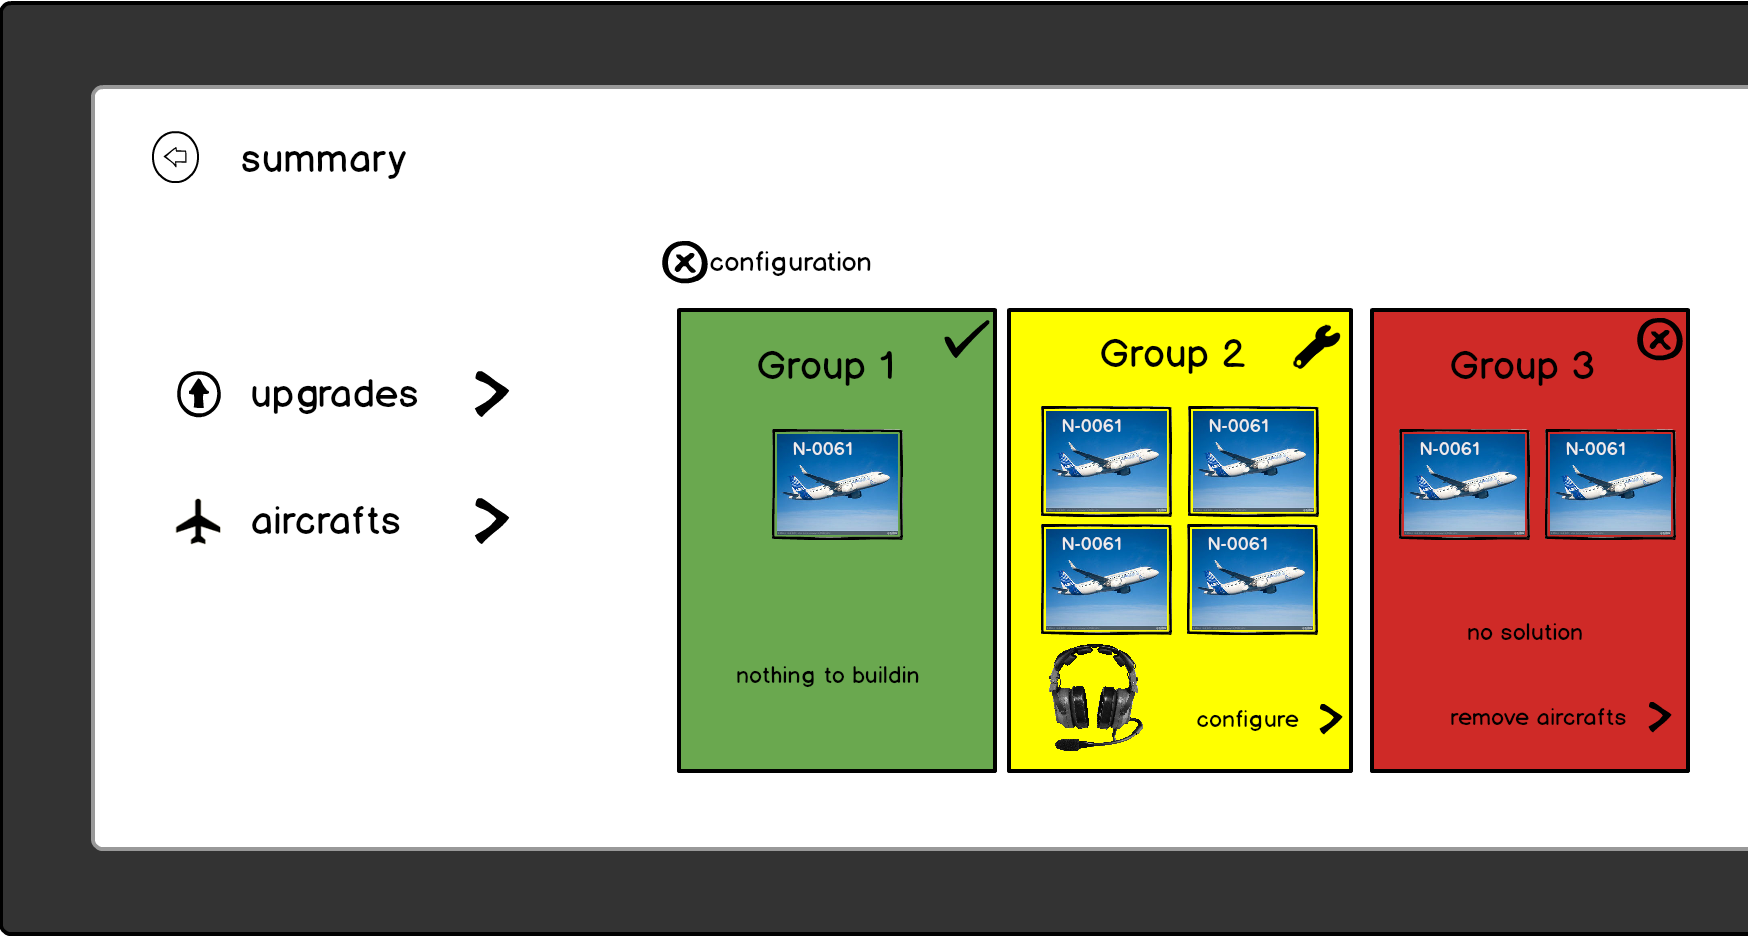
\includegraphics[width=\hsize]{images/configuration_entwurf}
\caption{Darstellung der Konfigurationsergebnisse}
\label{confSketch}
\end{figure}
 Für die Unterscheidung der verschiedenen Konfigurationsstatus werden verschiedene Farben verwendet (siehe Abbildung \ref{confSketch}). Die Darstellung erfolgt nach der Ampel Semantik. Rot bedeutet in diesem Zusammenhang, dass die Konfiguration für bestimmte Flugzeuge nicht durchführbar ist. Bei Gelb müssen Alternativen ausgewählt werden, damit der Grüne Status einer vollständigen Konfiguration für diese Gruppe erreicht wird. Die einzelnen Kacheln der Konfigurationsgruppen erhalten zusätzliche Icons, anhand derer ebenfalls eine Identifikation des Status abgelesen werden kann. Bei der Auswahl einer Konfigurationsgruppe gelangt man in die Alternativenauswahl. \par
 
 Die Seite für die Auswahl der Alternativen enthält eine kleine Zusammenfassung der Upgrades und Flugzeuge. Für jede Alternative wird eine selektierbare Kachel angezeigt. Nach der Auswahl wird der Status der Konfigurationsgruppe geändert und die Konfiguration kann abgeschlossen werden, wenn alle Gruppen grün sind.

\subsection{Weitere Ansichten}
Der Entwurf für die Hautfunktionen Upgradeauswahl, Flugzeugauswahl und Konfigurationsergebnisdarstellung ist abgeschlossen. Für die Umsetzung der Funktionalen-Anforderungen müssen weitere Ansichten hinzugefügt werden. Damit ein Speichern und Laden (F5) ermöglicht wird, soll eine Startseite verwendet werden. \par 
\begin{figure}
\centering
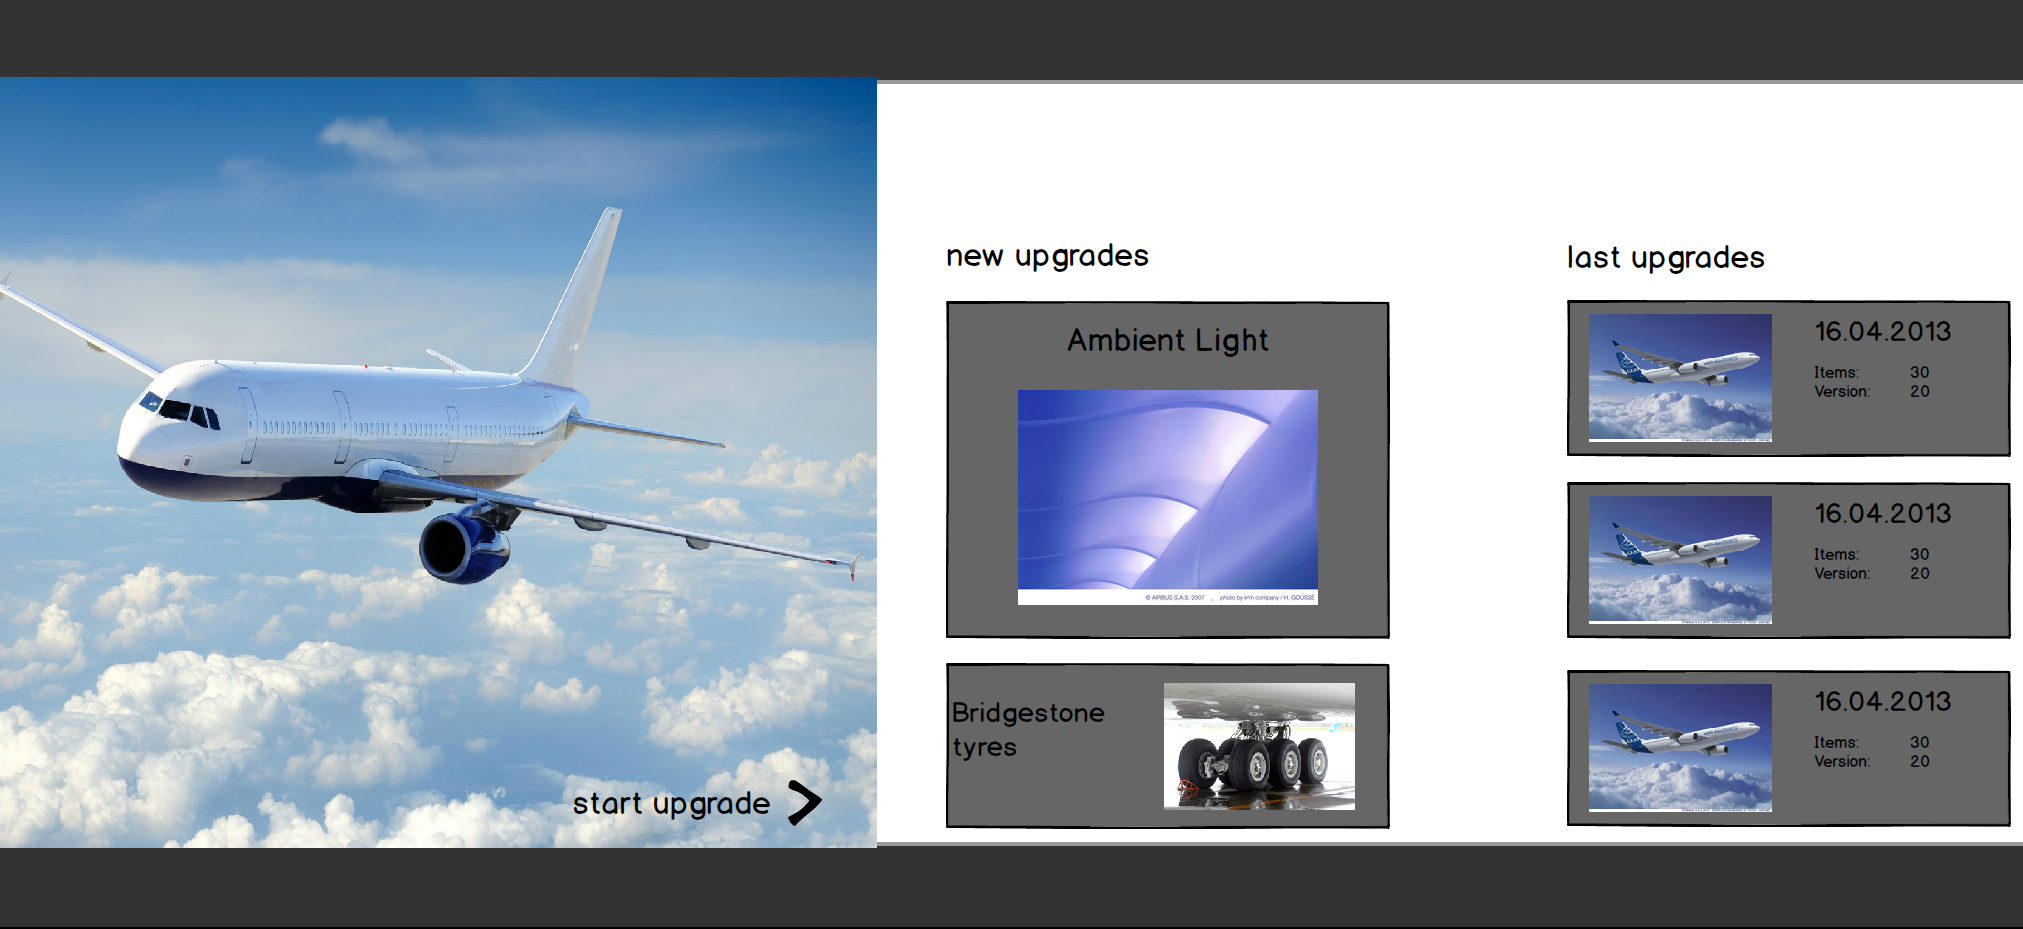
\includegraphics[width=\hsize]{images/start_entwurf}
\caption{Entwurf der Startseite}
\label{startSketch}
\end{figure}
Diese ist bereits im modellierten Workflow vorgesehen. Von der Startseite aus gelangt man in eine neue Konfiguration oder kann eine Vorhandene laden. Sie wird beim Start der Anwendung angezeigt. Somit ist diese Ansicht bei jeder Verwendung der App zu sehen. Aus diesem Grund ist das Design der Startseite wichtig. \par

 Die Idee ist eine kundenspezifische Startseite. Dies sorgt für eine Dynamik beim Anzeigen der Seite. Der Inhalt ist vom jeweiligen Kunden abhängig. Dies wird zuerst durch ein kundenspezifisches Bild zu Beginn erreicht (siehe Abbildung \ref{startSketch}). Bei der Auswahl des Bildes wird eine neue Konfiguration gestartet. Die Größe wird so gewählt, dass die letzten Konfigurationen erst durch ein scrollen komplett angezeigt werden. Hierdurch wird die Hauptfunktion schneller zugänglich und  die Microsoft Richtlinien der Konzentration auf das Wesentliche berücksichtigt. Als zweites Merkmal des Kunden wird das Logo der Fluggesellschaft am oberen linken Rand angezeigt. Für einen schnelleren Einstieg in die Anwendung werden neue oder für die Fluggesellschaft interessante Upgrades zusätzlich auf der Startseite angezeigt. Bei einem Klick auf diese Kachel wird die Detail Seite geöffnet, so dass mehr Informationen angezeigt werden und eine Auswahl möglich ist. 
\par 

Für die Umsetzung der Funktionalen Anforderung F6, die ein Filtern der Anwendungsdaten spezifiziert, wird eine weitere Ansicht benötigt. Die Daten sind in der Flugzeugauswahl und in der neuen Startseite auf einen Kunden beschränkt. Andere Datensätze werden nicht benötigt.  Das Problem mit der Filterung kann aus diesem Grund mit einer Kundenauswahl gelöst werden. Diese Auswahl stellt im Anschluss alle kundenspezifischen Daten der Anwendung bereit und erfüllt die Anforderung eines Filters. \par 

Die Ansicht für die Auswahl der Kunden wird analog zu der Flugzeugauswahl gestaltet. Es wird hier ebenfalls für jeden Kunden eine eigene Kachel angezeigt. Diese sind im Grid angeordnet. Eine Einteilung in Kategorien erfolgt Alphabetisch. Im Anwendungsbeispiel sind sehr viele Kunden vorhanden. Damit eine schnelle Auswahl erfolgen kann, wird der Semantische Zoom in der Ansicht verwendet. Die Kategorisierung erfolgt über das Alphabet. Es kann jedem Buchstaben ein Kunde zugeordnet werden. Nach der Auswahl eines Datums werden die kundenspezifischen Anwendungsdaten auf das mobile Endgerät geladen und können anschließend beim Kunden "'offline"' verwendet werden. \par 

Die zweite Filterung der Daten wird über die Programmauswahl realisiert. Diese Auswahl wird beim Starten einer neuen Konfiguration von der Startseite aus aufgerufen. Der Programmfilter wählt den richtigen Produktkatalog aus und verringert die Menge der vorhandenen Flugzeuge. Bei der visuellen Darstellung der Ansicht werden die vier möglichen Programme angezeigt. Damit der Kunde die Programmauswahl versteht, wird für jedes Programm ein passendes Flugzeugbild gewählt. Für die Umsetzung der "'Content over Chrome"' Richtlinie erhalten die vier Kacheln eine Bildschirmfüllende Größe, so dass die Auswahl mit Touch vereinfacht wird.


\section{Navigation und Bedienung}
Alle benötigten Ansichten sind den Anforderungen entsprechend konzipiert. Damit die Anforderung einer einfachen Bedienung (N1) erfüllt ist, muss ein passendes Navigationskonzept erstellt werden. Die Navigation unterstützt den Benutzer, indem es Fehler bei der Anwendung verzeiht. Hierzu gehört beispielsweise ein schnelles zurückspringen nach einer falschen Auswahl. Weiterhin muss ein schneller Ablauf des normalen Anwendungsfalls unterstützt werden. Der modellierte Workflow ist die Ausgangsbasis der Navigation. Dieser wird mit den zusätzlichen Ansichten und neuen Navigationsmöglichkeiten erweitert. \par 

\subsection{Navigationsverlauf}
\begin{figure}
\centering
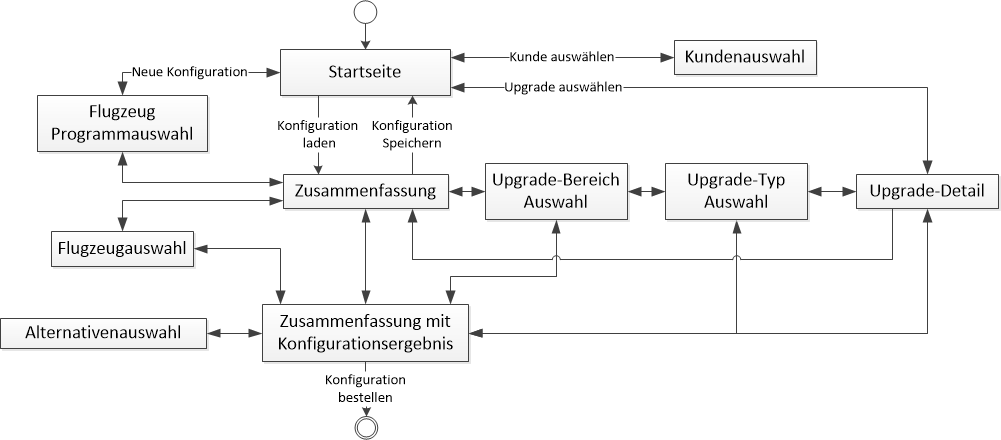
\includegraphics[width=\hsize]{images/workflow_navigation}
\caption{Navigation in der App}
\label{appNavigation}
\end{figure}
Abbildung \ref{appNavigation} zeigt die Möglichkeiten bei der Navigation. Es wird dabei eine hierarchische Struktur verwendet. Der Ursprungspunkt der Anwendung ist die Startseite. Von ihr können die vier Ansichten Programmauswahl, Zusammenfassung, Upgradedetail und Kundenauswahl erreicht werden.  Nach der Auswahl eines Kunden werden die Kundendaten geladen und es erfolgt ein Rücksprung zur Startseite. Nach Auswahl der drei anderen Möglichkeiten ist das Ziel die Zusammenfassung zu erreichen. Dies wird bei einer neuen Konfiguration erst nach der Auswahl eines Programms möglich. Bei der Selektion eines Upgrades wird von der Detailseite zurückgesprungen. Aus der Zusammenfassung kann in jede Hauptfunktion navigiert werden. Damit ist immer eine Ausgangsbasis vorhanden, anhand deren der Benutzer sich orientieren kann. Wenn sowohl Flugzeuge, als auch Upgrades ausgewählt sind, werden die Konfigurationsergebnisse in der Zusammenfassung angezeigt. Nachdem die benötigten Alternativen ausgewählt wurden, kann der Konfigurationsprozess durch die Bestellung abgeschlossen werden.
 
\subsection{Bedienelemente}
Damit die oben genannten Navigationsmöglichkeiten umgesetzt werden können, müssen passende Bedienelemente der Zielplattform ausgewählt werden. Hierzu werden folgende vier Möglichkeiten der Navigation eingesetzt: \par

\textbf{Auswahl durch Kacheln:} Zu den Hauptfunktionen der Anwendung wird mit großen Auswahlflächen navigiert. Diese besitzen ein aussagekräftiges Icon und werden direkt auf der Oberfläche angezeigt (siehe Entwürfe).  

\textbf{Obere AppBar:} Für die Navigation zu allen wichtigen Ansichten wird zusätzlich eine Möglichkeit in der oberen AppBar gegeben. Über dieses Bedienelement kann zu der Startansicht, Flugzeugauswahl, Upgradeauswahl und Zusammenfassung navigiert werden (Abbildung \ref{upperApp}). Diese Navigationsmöglichkeit ist in jeder Ansicht möglich und hilft dem erfahrenen Benutzer bei einer schnellen Bedienung (N2). \par
\begin{figure}[H]
\centering
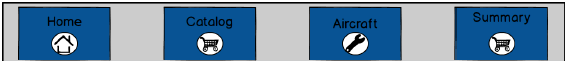
\includegraphics[width=\hsize]{images/UpperAppBar}
\caption{Obere AppBar für die Navigation}
\label{upperApp}
\end{figure}
\textbf{Untere AppBar:} Die Kundenauswahl ist nur für den Vertriebsexperten oder den Hersteller von Interesse. Aus diesem Grund wird die Navigation von der Startseite aus über die untere AppBar (siehe \ref{lowerApp}) ermöglicht.  Weiterhin wird diese Leiste für ein schnelles Navigieren von der Detailansicht zur Zusammenfassung verwendet . Nach der Auswahl eines Upgrades wird durch einen Klick auf den entsprechenden Menüeintrag (rechter Button im Bild) in der unteren AppBar  der Auswahlvorgang abgeschlossen und es erfolgt eine Navigation zur Zusammenfassung.
\begin{figure}[H]
\centering

\includegraphics[width=\hsize]{images/LowerAppBar}
\caption{Untere AppBar für die Navigation}
\label{lowerApp}
\end{figure}
\textbf{Zurück Button:} In jeder Ansicht, außer der Startseite, wird dem Benutzer das Zurückkehren zur vorigen Ansicht ermöglicht. Hierdurch kann eine unabsichtliche Navigation schnell rückgängig gemacht werden.

\section{Expertenmodus}
Beim Entwurf der Ansichten in Kapitel \ref{chapter_4} ist die Anforderung einer schnellen Bedienung mit dem Navigationskonzept umgesetzt worden. Damit nach der Heuristik einer flexiblen Nutzung weitere Möglichkeiten bei der Anwendung existieren, werden bei der Implementierung weitere Bedienelemente hinzugefügt. Bei diesen neuen Elementen ist es wichtig, dass diese nicht im Vordergrund stehen. Vielmehr sind diese erst nach dem Durchführen von bestimmten Aktionen für den Anwender sichtbar. Diese Maßnahmen haben das Ziel einen Expertenmodus zu etablieren.

\subsection{Flip View}
Im neuen Navigationsworkflow (siehe \ref{appNavigation}) muss für die Auswahl eines Upgrades mehrere Vorselektionen durchlaufen werden. Dieser Mechanismus ist für den Kunden ideal, da er so den Aufbau des Produktes, sowie die einzelnen Möglichkeiten versteht. Der Experte, der den Aufbau kennt und genau weiß, was er will, ist dies mit der Zeit anstrengend. An dieser Stelle muss eine weitere Möglichkeit geschaffen werden, die für den Experten geeignet ist. 

\subsection{Semantischer Zoom}
Die Entwürfe für die Kunden- und Flugzeugauswahl sehen die Verwendung des Semantischen Zooms vor. 
